% !TeX encoding = UTF-8

% 载入 SJTUThesis 模版
\documentclass[degree=bachelor, zihao=5]{sjtuthesis}
% 选项
%   degree=[doctor|master|bachelor|course],   % 可选(默认:doctor),学位类型
%   zihao=[-4|5],                             % 可选(默认:5),正文字号大小
%   language=[chinese|english],               % 可选(默认:chinese),论文的主要语言
%   review,                                   % 可选(默认:关闭),盲审模式
%   [twoside|oneside]                         % 可选(默认:twoside),单双页模式

% 论文基本配置,加载宏包等全局配置
% !TEX root = ./main.tex

\sjtusetup{
  %
  %******************************
  % 注意:
  %   1. 配置里面不要出现空行
  %   2. 不需要的配置信息可以删除
  %******************************
  %
  % 信息录入
  %
  info = {%
    %
    % 标题
    %   可使用“\\”命令手动控制换行
    %
    title           = {DNA分子通信系统的系统模型研究},
    title*          = {A Study of Systems Modeling in DNA-Based Molecular Communications},
    %
    % 关键词
    %
    keywords        = {DNA信息分子发送器, 微观分子通信实验平台, 微观DNA分子通信建模},
    keywords*       = {DNA Information Molecule Transmitter, 
    Experimental Platform of Micro Molecular Communication, Micro DNA Molecular Communication Modeling},
    %
    % 姓名
    %
    author          = {孙文韬},
    author*         = {Wentao\quad{}Sun},
    %
    % 指导教师
    %
    supervisor      = {闫浩},
    supervisor*     = {Hao Yan},
    %
    % 副指导教师
    %
    % assisupervisor  = {某某教授},
    % assisupervisor* = {Prof. Uom Uom},
    %
    % 学号
    %
    id              = {516030910265},
    %
    % 学位
    %   本科生不需要填写
    %
    degree          = {工学学士},
    degree*         = {Bachelor of Engineering},
    %
    % 专业
    %
    major           = {测控技术与仪器},
    major*          = {Measurement and Control Technology and Instrument Science},
    %
    % 所属院系
    %
    department      = {仪器科学与工程系},
    department*     = {Depart of Instrument Science and Engineering},
    %
    % 课程名称
    %   仅课程论文适用
    %
    coursename      = {某某课程},
    %
    % 答辩日期
    %   使用 ISO 格式;默认为当前时间
    %
    % date            = {2014-12-17},
    %
    % 资助基金
    %
    % fund  = {
    %           {国家 973 项目 (No. 2025CB000000)},
    %           {国家自然科学基金 (No. 81120250000)},
    %         },
    % fund* = {
    %           {National Basic Research Program of China (Grant No. 2025CB000000)},
    %           {National Natural Science Foundation of China (Grant No. 81120250000)},
    %         },
  },
  %
  % 格式设置
  %
  format = {%
    %
    % 本科论文页眉 logo 颜色
    %   默认为黑色
    %
    % header-logo-color = red,
  },
  %
  % 名称设置
  %
  name = {%
    % publications      = {攻读学位期间完成的论文},
  },
}

% 参考文献支持宏包
\usepackage[backend=biber,style=gb7714-2015,gbpub=false,gbpunctin=false]{biblatex}
% 导入参考文献数据库
\addbibresource{bibdata/thesis.bib}

% 定义图片文件目录与扩展名
\graphicspath{{figures/}}
\DeclareGraphicsExtensions{.pdf,.eps,.png,.jpg,.jpeg}

% 确定浮动对象的位置,可以使用 [H],强制将浮动对象放到这里(可能效果很差)
\usepackage{float}

% 固定宽度的表格
\usepackage{tabularx}

% 表格中支持跨行
\usepackage{multirow}

% 表格中数字按小数点对齐
\usepackage{dcolumn}
\newcolumntype{d}[1]{D{.}{.}{#1}}

% 附带脚注的表格
\usepackage{threeparttable}

% 算法环境宏包
\usepackage[ruled,vlined,linesnumbered]{algorithm2e}
% \usepackage{algorithm}

% 代码环境宏包
\usepackage{listings}
\lstnewenvironment{codeblock}[1][]
  {\lstset{style=lstStyleCode,#1}}{}

% 国际单位制宏包
\usepackage{siunitx}

% 定理环境宏包
\usepackage{ntheorem}
% \usepackage{amsthm}

% 绘图宏包
\usepackage{tikz}

% 化学方程式宏包
\usepackage[version=4]{mhchem}

%tikz宏包
\usepackage{tikz}

% 一些文档中用到的 logo
\usepackage{hologo}
\newcommand{\XeTeX}{\hologo{XeTeX}}
\newcommand{\BibLaTeX}{\textsc{Bib}\LaTeX}

% 借用 ltxdoc 里面的几个命令。
\def\cmd#1{\cs{\expandafter\cmd@to@cs\string#1}}
\def\cmd@to@cs#1#2{\char\number`#2\relax}
\DeclareRobustCommand\cs[1]{\texttt{\char`\\#1}}

\newcommand*{\meta}[1]{{%
  \ensuremath{\langle}\rmfamily\itshape#1\/\ensuremath{\rangle}}}
\providecommand\marg[1]{%
  {\ttfamily\char`\{}\meta{#1}{\ttfamily\char`\}}}
\providecommand\oarg[1]{%
  {\ttfamily[}\meta{#1}{\ttfamily]}}
\providecommand\parg[1]{%
  {\ttfamily(}\meta{#1}{\ttfamily)}}
\providecommand\pkg[1]{{\sffamily#1}}

% 自定义命令

% E-mail
\newcommand{\email}[1]{\href{mailto:#1}{\texttt{#1}}}

% hyperref 宏包在最后调用
\usepackage{hyperref}


\begin{document}

%TC:ignore

% 无编号内容:中英文论文封面、授权页
\maketitlepage
\makeorigpage*
\makeauthpage[scans/authorization.pdf]

% 使用罗马数字对前言编号
\frontmatter

% 摘要
% !TEX root = ../main.tex

\begin{abstract}
  中文摘要应该将学位论文的内容要点简短明了地表达出来,应该包含论文中的基本信息,
  体现科研工作的核心思想。摘要内容应涉及本项科研工作的目的和意义、研究方法、研究
  成果、结论及意义。注意突出学位论文中具有创新性的成果和新见解的部分。摘要中不宜
  使用公式、化学结构式、图表和非公知公用的符号和术语,不标注引用文献编号。硕士学
  位论文中文摘要字数为 500 字左右,博士学位论文中文摘要字数为 800 字左右。英文摘
  要内容应与中文摘要内容一致。

  摘要页的下方注明本文的关键词(4~6个)。
\end{abstract}

\begin{abstract*}
  Shanghai Jiao Tong University (SJTU) is a key university in China. SJTU was
  founded in 1896. It is one of the oldest universities in China. The University
  has nurtured large numbers of outstanding figures include JIANG Zemin, DING
  Guangen, QIAN Xuesen, Wu Wenjun, WANG An, etc.

  SJTU has beautiful campuses, Bao Zhaolong Library, Various laboratories. It
  has been actively involved in international academic exchange programs. It is
  the center of CERNet in east China region, through computer networks, SJTU has
  faster and closer connection with the world.
\end{abstract*}


% 目录、插图目录、表格目录
\tableofcontents
\listoffigures*
\listoftables*
\listofalgorithms* %算法

% 主要符号、缩略词对照表
% !TEX root = ../main.tex

\begin{nomenclature*}
\label{chap:symb}

\begin{longtable}{rl}
  $\epsilon$    & 介电常数 \\  
  $\mu$         & 磁导率 \\
\end{longtable}

\end{nomenclature*}


%TC:endignore

% 使用阿拉伯数字对正文编号
\mainmatter

% 正文内容
% !TEX root = ../main.tex

%先介绍做课题的目的和背景,再引出需要用到COMSOL来进行仿真,再介绍COMSOL


\chapter{绪论}
\section{课题研究背景}
本节简要介绍了分子通信的基本原理与发展现状。
介绍了课题组的微观分子通信实验平台的基本原理,
阐明了了本毕业设计工作的研究内容与研究意义。
\subsection{纳米网络的简述}
随着纳米技术的高速发展,研究者们现在可以
在纳米至微米尺度范围内制造能完成特定功能的结构,
这种微小结构被称为纳米机器(nanomachine)。
由于尺寸较小,单个纳米机器的功能非常有限,只能执行简单的任务
\cite{Weiss_©2003},严重限制了其应用于发展。为了解决这个问题,
纳米机器网络(简称纳米网络,nanonetwork)的概念被提出,
它将多个纳米机器互联、传递信息和彼此协调,扩展了纳米机器在信息采集、运算、储存
等方面的能力,进而使得整个纳米机器群体在更广的覆盖范围内执行更复杂和更精准的任务。
纳米网络在医疗卫生、工业制造、环境治理、国防建设等诸多领域有良好发展前景,
将广泛服务于我们的生产和生活中。

分子通信能够在复杂的生物环境和生物体中实现稳定而且可靠的信息传递,
同时具有生物兼容性好、不受收发器体积和能耗等限制等优点,被认为是组建
纳米网络,尤其是组建面向生物应用的纳米网络,最可行的通信方案之一
\cite{Suda05exploratoryresearch}。
\subsection{分子通信的基本原理}
分子通信(molecular communication)
指的是以生物化学分子作为信息载体的通信技术\cite{Hiyama2010Molecular}。

分子通信作为地球上最古老、最普遍的通信机制之一,广泛存在于自然界。
无论是对简单的单细胞生物,还是对复杂的多细胞动植物来说,分子通信都是维持它们生命必不可少的一环。
例如,许多细菌都会对它们邻居分泌的信号分子(information molecular)做出反应,以协调彼此的行为,并影响它们自身的运动、
产生抗生素、生成孢子等行为,这被成为群体感应。同样的,信号分子(例如信息素)
也广泛的存在于从低等的昆虫到高等的哺乳动物的日常交流中,并深深的影响了它们的行为。
信息素由个体释放,并指导群体里的其他个体前往觅食地,警告同伴有潜在的危险,
以及协调其他各种行为。此外,在多细胞动物体内,细胞与细胞之间也通过信号分子进行通信,
以完成相应的生理功能。例如,我们人体的神经系统中的电信号的传递,就是由神经递质(一种信号分子)
的释放与接收来完成的;在内分泌系统中,内分泌系统会向循环系统释放激素分子,
它作为一种信号分子被远端的目标细胞(靶细胞)所接收,从而完成细胞间的通信,调控靶细胞的行为\cite{Atakan2014Molecular}。

人工分子通信系统基于这一种在自然界就广泛存在的通信方式,
对传统的通信设备进行改造,以生物化学分子作为信息载体
在发射器和接收器之间进行通信。
如图
~\ref{fig:molecular_communication_example}
所示,一个典型的分子通信的典型过程包含三个过程
\cite{基于扩散的分子通信与身体域纳米网络}:
1)发送器(Transmitter)
生成携带着特定编码信息的信息分子(Information Molecule);
2)被释放的信息分子通过流体(液体或气体)介质传送到接又称接收器(Receiver);
3)接收机基于接受到的信息分子的物理或化学特性,对信息进行解码。
\begin{figure}[H]
    \centering
    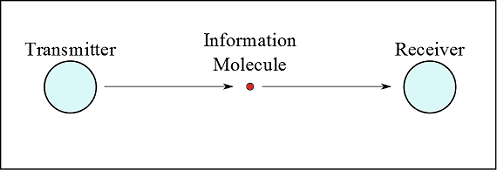
\includegraphics[scale=0.8]{simple model of molecular communication.png}
    \caption{分子通信示意图\cite{compic}}
    \label{fig:molecular_communication_example}
\end{figure}

为方便叙述,本文中“分子通信”特指人工分子通信,而非天然分子通信。

\subsection{分子通信的发展现状与面临挑战}
分子通信这个概念自2005年被提出以来\cite{Suda05exploratoryresearch},
就受到了相关领域研究者的密切关注,发展迅速,
在信道模型与容量分析、调制与解调技术、
信号检测技术、构架和协议设计等方面
已经有多种概念模型和基本框架被建立,
目前已经成为了纳米网络通信机制中非常重要的研究方向。

目前已经有研究成功的
实现了宏观的分子通信实验\cite{10.1007/978-81-322-1007-8_56},这证明了宏观分子通信的可行性。
然而建立纳米网络需要基于微观的分子通信系统,微观分子通信不单单是宏观分子通信
的缩小化,它们之间还存在较大的差别,因此宏观的分子通信实验还不能解决
纳米网络对微观分子通信的实验需求。

总的来说,分子通信的研究主要都集中在理论方面,缺乏实验研究,技术成熟度低。
造成这种现状的最主要的瓶颈问题是
缺少能执行稳定而连续信息传递的微观分子通信平台,使得大量的理论研究
成功无法通过实验进行验证,更进一步阻碍了纳米网络从理论向实际应用的推进,严重
限制了该领域的发展。所以,尽快突破微观分子通信实验平台这个瓶颈问题,已成为纳米网络与分子通信领域
的关注核心和基本共识\cite{Liu1999}。

其中DNA分子通信指的是以DNA为信息分子的分子通信系统。
在当前纳米机器研究中,DNA纳米机器是其中最具有可能迈向第三代
包含人工智能和纳米计算机在内的纳米机器种类\cite{McCutcheon2017}。
因此本课题组正在开展以DNA为信息载体、
以DNA纳米机器为通信主体的微观分子通信实验平台的研究,
为纳米网络提供第一个完整的微观分子通信实验平台,解决本领域瓶颈问题。

\section{课题研究目的及意义}
本毕业设计立足于课题组的现有的DNA分子通信实验平台,对其发送器部分开展理论研究。
我们实现的DNA信息分子的发送器,是一个宏观电信号到微观DNA信号的转化接口。
其主要原理是将锆离子$\ce{Zr^4+}$作为粘合剂胶水,
采用LbL(Layer-by-Layer,逐层)自组装技术在金薄膜表面固定完成多层DNA/$\ce{Zr^4+}$结构。
通过电化学反应执行多层DNA结构的分解与可控释放。
本课题组在先前实验中已经构建完成了基于DNA/$\ce{Zr^{4+}}$LbL自组装结构的
分子通信系统,该系统在外部电压控制下可以将DNA分子从发送机上释放到溶液中。
但对于该分子通信系统的系统模型研究还未开展。

而在所有理论研究中,系统模型是其他理论研究的基础。
首先,虽然目前大量不同的分子通信的理论模型被提出。
但是当前系统模型的研究成果均未经过实验验证其有效性。
更为重要的是,由于DNA的释放与接收机制与以往系统的不同,
因此本项目的DNA微观分子通信的系统模型不同于之前其他
微观分子通信的系统模型。
又由于领域内尚未开展DNA分子通信的研究,
因此需要根据DNA信息分子的释放与接收机制特点,
开展DNA微观分子通信系统模型的研究。

所以本文立足于实验平台,结合DNA微观分子通信特征,开展系统建模的研究。
在课题组实验的基础上,探究DNA受控释放的原理。
综合分子通信理论、电化学反应原理、化学动力学原理、扩散原理
等对DNA的受控释放过程进行建模与仿真。
根据仿真结果对影响该分子通信系统性能的参数进行
研究,并调整参数进行系统的优化。

该研究可以解决目前大量纳米网络与分子通信的理论研究亟需通过实验验证的问题,促
进纳米网络与分子通信的理论研究沿着正确的方向发展。
其次,也将为纳米网络与分子通信从理论研究向实际应用的迈进奠定关键的一步。
因此,无论从理论上还是实践上,本项目的研究都具有重要意义。           %引言
% !TEX root = ../main.tex
\chapter{DNA分子的释放过程简述}
\section{DNA/Zr$^{4+}$层层自组装结构}
\subsection{组装过程}
——用到的组装方法
\subsection{理化性质}
——介绍该结构的物理与化学性质
\section{层层自组装结构受控分解的原理}
\subsection{电信号激励下的电化学反应}
——通过电极电位表等客观条件,推断出通电后发生的电极反应
\subsection{Zr$^{4+}$水解过程}
——介绍Zr$^{4+}$水解相关的内容
\subsection{电场影响下DNA分子运动}
——介绍在浓度梯度力与电场力共同作用下DNA的行为
\subsection{反应过程总述}
——总结反应过程,插入反应过程图等
\section{基本控制方程}
\subsection{扩散定律}
——主要用到菲克定律,稀溶液中粒子的扩散。
\subsection{Nernst-Einstein 关系}
——得到物质化合价和迁移率与扩散率的关系\parencite{Ferrari1985}
\subsection{Nernst-Planck 方程}
——电化学系统中离子的运动,计算粒子通量
\subsection{化学反应速率方程}
——反应物浓度影响反应速度
\subsection{Butler-Volmer 方程}
——电极电势与电化学反应速率的关系

            %释放过程介绍
%% !TEX root = ../main.tex
\chapter{}
\section{}              %模型建立
% !TEX root = ../main.tex
\chapter{建模与仿真}

\section{求解过程的简述}
根据第二章中推导的反应过程,仿真的过程主要分为以下三步:

1)在COMSOL Multiphysics中,对通电时发生的电化学反应进行建模,得到阴极极板表面的平均$\ce{OH-}$浓度随
时间的变化曲线。

2)利用第1步得到的浓度变化随时间的变化曲线,在MATLAB中计算$\ce{Zr^4+}$的水解程度随时间的变化关系,
再根据$\ce{Zr^4+}$消耗与DNA释放这一正比关系,得到DNA的释放曲线。

3)利用第2步得到的数据,在COMSOL Multiphysics中,对DNA在电场力以及浓度梯度力作用下的扩散、迁移过程进行建模仿真。
\section{反应容器物理模型}
本课题组使用的反应容器为一个长度为$2cm$,直径为$1cm$的圆柱体。作为电极的金薄膜的规格为$20mm×6mm×1mm$。

如图~\ref{fig:container} 所示,根据上述数据,我们可以在COMSOL Multiphysics中完成对反应溶液的物理模型的建立。
由于电极材料为金,不参与反应,内部也考虑为等势体,所以我们只用考虑在溶液体系内发生的反应,在建模时只用对溶液
进行建模。
\begin{figure}[ht]
    \centering
    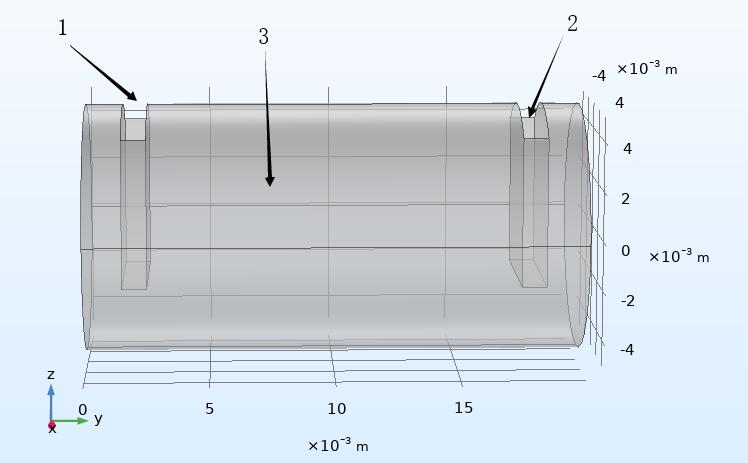
\includegraphics[scale=1]{container.jpg}\\
    1)阳极(Anode) 2)阴极(Cathode) 3)电解液(Electrolyte)
    \caption{反应容器物理模型}
    \label{fig:container}
\end{figure}

\section{电化学反应仿真}
\subsection{计算流程}
——介绍COMSOL Multiphysics的操作及计算过程
\subsection{结果与讨论}
——讨论结果以及参数影响等

\section{Zr$^{4+}$水解反应仿真}
\subsection{计算流程}
——介绍在MATLAB中计算水解量
\subsection{结果与讨论}
——讨论结果以及参数影响等

\section{DNA扩散过程仿真}
\subsection{计算流程}
——介绍COMSOL Multiphysics的操作及计算过程
\subsection{结果与讨论}
——讨论结果以及参数影响等             %仿真
% !TEX root = ../main.tex
\chapter{根据仿真结果对进行通信系统优化}

\section{控制电压释放曲线实现逐层释放}
——讨论如何控制电压释放曲线以实现逐层释放

\section{接收机位置与最大传输速度的关系}
——讨论接收机位置与传输速度的关系

\section{阈值影响}
%决定了一层膜释放的次数。可以求出单次激励对膜的最小消耗量。信号周期也会被限制。一层膜可否释放多次。             %讨论如何释放
% !TEX root = ../main.tex

\begin{summary}
针对分子通信领域缺少微观实验平台的瓶颈问题,
本课题组提出了以DNA为信息分子的微观分子通信实验平台
 ,并初步完成了其中关键部件的DNA信息分子的发送器与接收器的设计与实现
。然而,针对DNA分子通信,领域内并没有相关的理论研究。但是,
对实验平台的深入理解,离不开理论研究的指导。针对这个问题,
本毕业设计立足于课题组的现有的DNA分子通信实验平台,对其中DNA信息分子发送器部分开展理论研究。\\

首先,我们融合化学、物理学科的知识,利用COMSOL Multiphysics与MATLAB软件,基于电化学反应原理、化学动力学原理、粒子自由扩散与带电粒子在电场辅助下自由扩散的原理,获得了DNA信息分子发送器的三维理论模型。其次,我们利用获得的DNA信息分子发送器模型,研究了关键参数对DNA发送过程的影响,包括:激励信号与接收机位置等,并分析了关键系统参数对信息传播速度、抗干扰能力、总发送量这三个性能的影响。通过本工作的研究,课题组深入理解了DNA信息分子发送器的特征,指明了优化DNA信息分子发送器的具体方向。对进一步推进本课题组的微观分子通信实验平台的研究具有重要意义。\\

本工作的主要研究结果包含如下几个方面:

1)通过学习,了解了分子通信领域的发展现状与分子通信的基本原理。 

2)通过调研与阅读多学科文献,学习、归纳并总结了DNA信息分子发送器中关键的多层DNA结构的组装过程
、理化性质以及DNA分子的扩散运动运动过程。通过自己的理解与调研
,详细分析与讨论了DNA信息分子分解与释放过程中的电化学反应、水解反应、
电迁移及扩散过程,并最终提出DNA/$\ce{Zr^4+}$多层结构的分解与释放的原理。并
将上述多个过程表达为对应的理论方程。

3)利用两个软件,COMSOL Multiphysics 与 MATLAB,对上述DNA信息分子发送过
程进行数值仿真,仿真结果与课题组的实验数据符合度好,证明了所提出的模型的准确性与有效性。
也验证了利用COMSOL Multiphysics 与 MATLAB对电极反应、水解反应、
电泳等多个过程共同作用的仿真可以用于对DNA分子通信系统的建模。

4)对DNA信息分子发送器的系统特征进行研究,深入理解了DNA信息分子发送器的
特征,指明了优化DNA信息分子发送器的具体方向。关键结论包括:

$\bullet$讨论了激励电压信号的强度与持续时间对DNA信息分子发送过程的影响。不考虑电解热效应的情况下,
激励电压越高,系统抗码间串扰的能力越强。激励时长越短,系统抗码间串扰的能力越强。激励信号需要具备持续时间较短
、激励电压较高的特性,高电压的脉冲函数是一个理想的信号源。

$\bullet$讨论了接收机位置对系统性能的影响,获得信道中不同位置初的DNA浓度变化曲线并研究了DNA信息分子发送器
的阈值。接收机距离阴极越近,DNA浓度达到峰值的时间越短,峰值强度越大。接收机距离越短,信号传输效果越好。
短时长的信号的激励下,相同位置处,DNA浓度峰值会更早到达,峰值相对于整条曲线也会更突出。
在距离阴极 0.5$mm$的地方,我们可以达到54.5$bit/min$的最大通信速率;
在距离阴极 4.5$mm$处,我们可以达到16.7$bit/min$的最大通信频率,而在距离阴极9.5$mm$处,最大通信频率只有3.2$bit/min$。
数据说明了,基于自由扩散的通信系统,
不适合远距离通信。接收机放置在距发送机5$mm$以内这一范围内时,能达到一个较快的传输速度,
而且抗干扰能力强。在超过7$mm$这一范围后,
信号间隔必须增加到数十秒,以抑制码间串扰,而且其抗码间串扰的能力能力也会下降。

$\bullet$综合考虑平衡常数,在$\ce{OH-}$存在时,$\ce{Zr^4+}$水解反应都会发生,
由于反应速度与$c_{\ce{OH-}}$的4次方成正比,所以低$\ce{OH-}$浓度时,
反应速度极慢,在所观测的时间尺度下,可以认为不施加激励电压时反应不发生。
电化学反应的电压阈值应为2.17$V$。但实际条件下,由于电极阻抗、溶液电导率等因素的影响,
可能需要更大的电压来启动此反应。通过对激励电压与时长的控制,一个DNA/$\ce{Zr^4+}$单层可以被多次释放,
在激励电压为5$V$,激励时长为1$s$的信号作用下,每一层DNA/$\ce{Zr^4+}$单层最多可以释放6次。


\end{summary}
                %结论与展望

%TC:ignore

% 使用英文字母对附录编号
\appendix

% 附录内容,本科学位论文可以用翻译的文献替代。
%% !TEX root = ../main.tex

\chapter{Maxwell Equations}

选择二维情况,有如下的偏振矢量:
\begin{subequations}
  \begin{align}
    {\bf E} &= E_z(r, \theta) \hat{\bf z}, \\
    {\bf H} &= H_r(r, \theta) \hat{\bf r} + H_\theta(r, \theta) \hat{\bm\theta}.
  \end{align}
\end{subequations}
对上式求旋度:
\begin{subequations}
  \begin{align}
    \nabla \times {\bf E} &= \frac{1}{r} \frac{\partial E_z}{\partial\theta}
      \hat{\bf r} - \frac{\partial E_z}{\partial r} \hat{\bm\theta}, \\
    \nabla \times {\bf H} &= \left[\frac{1}{r} \frac{\partial}{\partial r}
      (r H_\theta) - \frac{1}{r} \frac{\partial H_r}{\partial\theta} \right]
      \hat{\bf z}.
  \end{align}
\end{subequations}
因为在柱坐标系下,$\overline{\overline\mu}$ 是对角的,所以 Maxwell 方程组中电场
$\bf E$ 的旋度:
\begin{subequations}
  \begin{align}
    & \nabla \times {\bf E} = \upi \omega {\bf B}, \\
    & \frac{1}{r} \frac{\partial E_z}{\partial\theta} \hat{\bf r} -
      \frac{\partial E_z}{\partial r}\hat{\bm\theta} = \upi \omega \mu_r H_r
      \hat{\bf r} + \upi \omega \mu_\theta H_\theta \hat{\bm\theta}.
  \end{align}
\end{subequations}
所以 $\bf H$ 的各个分量可以写为:
\begin{subequations}
  \begin{align}
    H_r &= \frac{1}{\upi \omega \mu_r} \frac{1}{r}
      \frac{\partial E_z}{\partial\theta}, \\
    H_\theta &= -\frac{1}{\upi \omega \mu_\theta}
      \frac{\partial E_z}{\partial r}.
  \end{align}
\end{subequations}
同样地,在柱坐标系下,$\overline{\overline\epsilon}$ 是对角的,所以 Maxwell 方程
组中磁场 $\bf H$ 的旋度:
\begin{subequations}
  \begin{align}
    & \nabla \times {\bf H} = -\upi \omega {\bf D}, \\
    & \left[\frac{1}{r} \frac{\partial}{\partial r}(r H_\theta) - \frac{1}{r}
      \frac{\partial H_r}{\partial\theta} \right] \hat{\bf z} = -\upi \omega
      {\overline{\overline\epsilon}} {\bf E} = -\upi \omega \epsilon_z E_z
      \hat{\bf z}, \\
    & \frac{1}{r} \frac{\partial}{\partial r}(r H_\theta) - \frac{1}{r}
      \frac{\partial H_r}{\partial\theta} = -\upi \omega \epsilon_z E_z.
  \end{align}
\end{subequations}
由此我们可以得到关于 $E_z$ 的波函数方程:
\begin{equation}
  \frac{1}{\mu_\theta \epsilon_z} \frac{1}{r} \frac{\partial}{\partial r}
  \left(r \frac{\partial E_z}{\partial r} \right) + \frac{1}{\mu_r \epsilon_z}
  \frac{1}{r^2} \frac{\partial^2E_z}{\partial\theta^2} +\omega^2 E_z = 0.
\end{equation}

%% !TEX root = ../main.tex

\chapter{绘制流程图}

图~\ref{fig:flow_chart} 是一张流程图示意。使用 \pkg{tikz} 环境,搭配四种预定义节
点(\verb+startstop+、\verb+process+、\verb+decision+和\verb+io+),可以容易地绘
制出流程图。

\begin{figure}[!htp]
  \centering
  \resizebox{6cm}{!}{\begin{tikzpicture}[node distance=2cm]
    \node (pic) [startstop] {待测图片};
    \node (bg) [io, below of=pic] {读取背景};
    \node (pair) [process, below of=bg] {匹配特征点对};
    \node (threshold) [decision, below of=pair, yshift=-0.5cm] {多于阈值};
    \node (clear) [decision, right of=threshold, xshift=3cm] {清晰?};
    \node (capture) [process, right of=pair, xshift=3cm, yshift=0.5cm] {重采};
    \node (matrix_p) [process, below of=threshold, yshift=-0.8cm] {透视变换矩阵};
    \node (matrix_a) [process, right of=matrix_p, xshift=3cm] {仿射变换矩阵};
    \node (reg) [process, below of=matrix_p] {图像修正};
    \node (return) [startstop, below of=reg] {配准结果};
     
    %连接具体形状
    \draw [arrow](pic) -- (bg);
    \draw [arrow](bg) -- (pair);
    \draw [arrow](pair) -- (threshold);

    \draw [arrow](threshold) -- node[anchor=south] {否} (clear);

    \draw [arrow](clear) -- node[anchor=west] {否} (capture);
    \draw [arrow](capture) |- (pic);
    \draw [arrow](clear) -- node[anchor=west] {是} (matrix_a);
    \draw [arrow](matrix_a) |- (reg);

    \draw [arrow](threshold) -- node[anchor=east] {是} (matrix_p);
    \draw [arrow](matrix_p) -- (reg);
    \draw [arrow](reg) -- (return);
\end{tikzpicture}
}
  \bicaption{绘制流程图效果}{Flow chart}
  \label{fig:flow_chart}
\end{figure}


% 文后无编号部分
\backmatter

% 参考资料
\printbibliography[heading=bibintoc]

% 用于盲审的论文需隐去致谢、发表论文、参与项目、申请专利、简历

% 致谢
% !TEX root = ../main.tex

\begin{acknowledgements}
  感谢那位最先制作出博士学位论文 \LaTeX 模板的交大物理系同学!

  感谢 William Wang 同学对模板移植做出的巨大贡献!

  感谢 \href{https://github.com/weijianwen}{@weijianwen} 学长一直以来的开发和维
  护工作!

  感谢 \href{https://github.com/sjtug}{@sjtug} 以及
   \href{https://github.com/dyweb}{@dyweb} 对 0.9.5 之后版本的开发和维护工作!

  感谢所有为模板贡献过代码的同学们, 以及所有测试和使用模板的各位同学!

  感谢 \LaTeX 和 \href{https://github.com/sjtug/SJTUThesis}{\sjtuthesis},帮我节
  省了不少时间。
\end{acknowledgements}


% 发表论文、参与项目、申请专利、简历
% 盲审论文中,发表学术论文及参与科研情况等仅以第几作者注明即可,不要出现作者或他人姓名
%% !TEX root = ../main.tex

\begin{publications}
  \item Chen H, Chan C~T. Acoustic cloaking in three dimensions using acoustic metamaterials[J]. Applied Physics Letters, 2007, 91:183518.
  \item Chen H, Wu B~I, Zhang B, et al. Electromagnetic Wave Interactions with a Metamaterial Cloak[J]. Physical Review Letters, 2007, 99(6):63903.
\end{publications}

\begin{publications*}
  \item 第一作者. 中文核心期刊论文, 2007.
  \item 第一作者. EI 国际会议论文, 2006.
\end{publications*}

%% !TEX root = ../main.tex

\begin{achievements}
  \item 第一发明人,“永动机”,专利申请号202510149890.0
\end{achievements}

\begin{achievements*}
  \item 第一发明人,“永动机”,专利申请号XXXXXXXXXXXX.X
\end{achievements*}

%% !TEX root = ../main.tex

\begin{resume}
  \subsection*{基本情况}
    某某,yyyy 年 mm 月生于 xxxx。

  \subsection*{教育背景}
  \begin{itemize}
    \item yyyy 年 mm 月至今,上海交通大学,博士研究生,xx 专业
    \item yyyy 年 mm 月至 yyyy 年 mm 月,上海交通大学,硕士研究生,xx 专业
    \item yyyy 年 mm 月至 yyyy 年 mm 月,上海交通大学,本科,xx 专业
  \end{itemize}

  \subsection*{研究兴趣}
    \LaTeX{} 排版

  \subsection*{联系方式}
  \begin{itemize}
    \item 地址: 上海市闵行区东川路 800 号,200240
    \item E-mail: \email{xxx@sjtu.edu.cn}
  \end{itemize}
\end{resume}


% 中文学士学位论文要求在最后有一个英文大摘要,单独编页码,英文学士学位论文不需要
% !TEX root = ../main.tex

\begin{digest}
  Molecular communication is an important communication scheme to establish a nano-machine network, which can solve the current problem that the limited capacity of a single nanomachine makes it difficult to carry out any concrete applications. The nano-network built by molecular communication technology can enable the entire nano-machine group to perform more complex tasks in a wider range, which is beneficial to the development of nano-machine applications, such as micro-surgery through the cooperation of a large number of nano-machines or drug delivery inside the human body. Therefore, molecular communication is a promising research direction and has received extensive attention.\\

  At present, the main research work in the field of molecular communication is concentrated on theory. So far, there is no complete microscopic molecular communication experimental platform, which seriously limits the development of the field of molecular communication and becomes a bottleneck in this field. Aiming at the bottleneck in this field, our group proposed a micro-molecular communication experiment platform using DNA as the information molecule, and completed the transmitter and receiver of DNA information molecules, which are the key components of the experiment platform. However, there is no relevant theoretical research on DNA molecular communication in this field. However, a thorough understanding of the experimental platform is inseparable from the guidance of theoretical research.\\
  
  To solve the above problems, this work is based on the existing DNA molecular communication experimental platform of our group and carries out theoretical research on its transmitter part. The transmitter of DNA information molecules that we implemented is a conversion interface from macroscopic electrical signals to microscopic DNA signals. In this contribution we illustrate a simple layer-by-layer assembly strategy to immobilize DNA on the surface of gold thin film and to trigger the selective release of DNA upon the exclusive control ofexternal electric potential. The assembly of DNA-containing multilayer films is driven by coordination/electrostatic interactions between inorganic zirconium ion (Zr4+) and phosphate groups in the backbone of the DNA chain. Its main principle is to use zirconium ion Zr4+ as the adhesive glue, and use the layer-by-layer self-assembly technology to fix the multilayer DNA/Zr4+ structure on the surface of the gold film. The decomposition and controllable release of multilayer DNA structures are performed through electrochemical reactions. This work carries out complete mathematical modeling on the above DNA decomposition and release process. Specifically, we use the electrochemical reaction model, chemical kinetic model and particle free diffusion model in physics to study the overall process of decomposition, release and propagation of the DNA multilayer structure. Using two softwares, COMSOL Multiphysics and MATLAB, this process was studied and a three-dimensional model of DNA decomposition and release process was established. Using the obtained model, the influence of key parameters on the process of DNA decomposition and release was studied, and then the characteristics of the DNA information molecular transmitter were deeply understood, and the specific direction of optimizing the DNA information molecular transmitter was pointed out. It is of great significance to further promote the research of the micro-molecular communication experiment platform in our group.\\
  
  The main work of this work includes the following aspects:
  
  1) A brief introduction to the basic principles and development status of molecular communication. The basic principles of the micro-molecular communication experiment platform of our group were introduced, and the research content and significance of the graduation project work were clarified. The application example of the key software COMSOL Multiphysics of this work in the field of molecular communication is introduced.

  2) The assembly process and physical and chemical properties of the key multi-layer DNA structure in the DNA information molecular transmitter are introduced. The electrochemical reaction, hydrolysis reaction, electromigration and diffusion process during the decomposition and release of DNA information molecules are analyzed and discussed in detail. The theoretical equations expressing the above process and particle motion process are introduced and explained in detail.
  
  3) Using COMSOL Multiphysics, three-dimensional modeling and simulation were carried out on the electrochemical reaction, hydrolysis reaction, electromigration and diffusion process of DNA information molecule decomposition, release and propagation. The obtained DNA concentration curve data from our established model agrees with the previous experimental data. Thus correctness of the obtained model of our DNA information molecular transmitter is validated.
  
  4) Study the system characteristics of DNA information molecular transmitter. The influence of the intensity and duration of the excitation voltage signal on the transmission process of DNA information molecules is discussed, and the DNA concentration change curves at different positions in the channel are obtained and the threshold of the DNA information molecule transmitter is studied. In-depth understanding of the characteristics of DNA information molecular transmitter is achieved which points out the specific direction of optimization of our DNA information molecular transmitter,including:
  
  $\bullet$The influence of the intensity and duration of the excitation voltage signal on the transmission process of DNA information molecules is discussed. Without considering the thermal effect of electrolysis, the higher the excitation voltage is, the stronger the ability of the system to resist the intersymbol interference will be. The shorter the excitation time is, the stronger the system's ability to resist the intersymbol interference will be. The excitation signal needs to have the characteristics of short duration and high excitation voltage, thus a high voltage pulse function is an ideal signal source.
  
  $\bullet$The influence of receiver position on system performance is discussed. The closer the receiver is to the cathode, the shorter the time for DNA concentration to reach the peak value, and the greater the peak intensity. The shorter the receiver distance, the better the signal transmission effect. Under the stimulation of short-term and long-term signals, the peak of DNA concentration will arrive earlier at the same position, and the peak will be more prominent than the whole curve. At a distance of 0.5mm from the cathode, we can reach the maximum communication rate of 0.909hz; at a distance of 4.5mm from the cathode, we can reach the maximum communication frequency of 0.2778hz, while at a distance of 9.5mm from the cathode, the maximum communication frequency is only 0.05348hz. The data shows that the communication system based on free diffusion is not suitable for long-distance communication.
  
  $\bullet$When the receiver is placed within the range of 5mm from the transmitter, it can achieve a faster transmission speed and strong anti-interference ability. After the range of 7mm, the signal interval must be increased to tens of seconds to suppress the inter code interference, and its ability to resist the inter code interference will also be reduced. 
  Considering the equilibrium constant, in the presence of OH-, the hydrolysis reaction of Zr4+ will occur. Because the reaction speed is proportional to the fourth power of COH -, the reaction speed is extremely slow at low OH - concentration. Under the observed time scale, it can be considered that the reaction will not occur without applying the excitation voltage. The voltage threshold of electrochemical reaction should be 2.17v. However, under the actual conditions, due to the influence of electrode impedance, solution conductivity and other factors, more voltage may be needed to start the reaction. By controlling the excitation voltage and duration, a DNA / Zr4 + monolayer can be released many times. Under the signal of excitation voltage of 5V and excitation duration of 1s, each layer of Zr4 + / DNA monolayer can be released six times at most.


\end{digest}


%TC:endignore

\end{document}
